% !TEX root = ../oddp.tex

\section{Cyclic straightenings and subdivisions of simplices}\label{section:atlast}

\subsection{Barycentric subdivisions}\label{s:assembly}

Recall that the barycentric subdivision $\sd \partial\simplex^n$ of the boundary of the standard simplex $\simplex^n$ is the simplicial complex that has one vertex for each non-empty face of $\simplex^n$ and one face $(\tau_0,\dots,\tau_k)$ of dimension $k$ for every ascending chain $\tau_0 \subset \tau_1\subset\dots \subset \tau_k$ of simplices of $\partial \simplex^n$. We will denote the face $\tau_0 \subset \dots \subset \tau_k)$ as $(\bar{\tau}_0|\bar{\tau}_1|\dots|\bar{\tau}_k)$, where $\bar{\tau}_i = \tau_i\smallsetminus \tau_{i-1}$ is the face such that the geometric join $\bar{\tau}_i\star \tau_{i-1}$ is the face $\tau_i$. With this notation, the differential on $\cadenas(\sd \partial \simplex^n)$ becomes
\[
\partial(\bar{\tau}_0|\bar{\tau}_1|\dots|\bar{\tau}_k) = \sum_{i=0}^{k-1} (-1)^i(\bar{\tau}_0|\dots|\bar{\tau}_i\star \bar{\tau}_{i+1}|\dots |\bar{\tau}_k) + (-1)^k (\bar{\tau}_0|\dots|\bar{\tau}_{k-1}).
\]

The \emph{pair barycentric subdivision} $\Psd \partial\simplex^n$ of $\partial \simplex^n$ is a cubulation of $\partial \simplex^n$ with the same vertices as $\sd \partial \simplex^n$ and one face for each pair $(b,a)$ of faces of $\partial\simplex^n$ such that $b \subset a$ (cf. \cite{Rounds2010}). Geometrically, that face is the union of all the faces of dimension $|a|-|b|$ of the barycentric subdivision that correspond to ascending chains $b = \tau_0 \subset \dots \subset \tau_k= a$. Interpreting $b$ as a dual cochain, its chain complex $\cadenas(\Psd \partial\simplex^n)$ is isomorphic to the tensor product $\cochains(\partial\simplex^n) \ot \chains(\partial\simplex^n)$ modulo the pairs $b \ot a$ such that the support of $b$ is not contained in $a$.


There are chain maps
\[
\xymatrix{
	&\susp{-n-1}\chains(\partial\simplex^n) \ot \chains(\partial\simplex^n)\ar[d]^h& \\
	\cadenas(\partial\simplex^n)\ar[r]^{s_*^{\simplex}}\ar@/_2.0pc/[rr]^{s_*} & \cadenas(\Psd \partial\simplex^n)\ar[r]^{s^{\Psd}_*} & \cadenas(\sd\partial\simplex^n)
}
\]
defined as follows: if $[a_0,\dots,a_{k-1}]\in \cadenas(\partial\simplex^n)$ is an ordered representative of a generator,
\begin{align*}
	s_*([a_0,\dots,a_{k-1}]) &= \sum_{\perm\in \Sigma_{k}} (-1)^{\sign{\perm}}(a_{\perm(0)}|a_{\perm(1)}|\dots|a_{\perm(k-1)}),
	\\
	s_*^{\simplex}([a_0,\dots,a_{k-1}]) &= (-1)^{k}\sum_{j=0}^{k-1} (a_j) \ot [a_0,\dots,a_{k-1}].
\end{align*}
If $b = (b_0,\dots,b_{m-1})\in \cochains(\partial\simplex^n)$ and $a = [b_0,\dots,b_{m-1},c_0,\dots,c_{\ell-1}]\in \chains(\partial\simplex^n)$ with $k = m+\ell$, then
\begin{equation}\label{eq:sP}
	s_*^{\Psd}(b \ot a) = (-1)^{\ell+1}\sum_{\perm\in \Sigma_{k+1}} (-1)^{\sign{\perm}} (b|c_{\perm(0)}|c_{\perm(1)}|\dots|c_{\perm(\ell-1)})
\end{equation}
Notice that the letter $b$ plays a different role in each side: on the left, it is a dual generator of the normalized cochain complex, thus it makes sense to permute its entries changing the generator by a sign. On the right, $b$ is a vertex of $\sd\partial\simplex^n$.

\begin{remark}
	Let $\twist \colon A \ot B \to B \ot A$ the chain map that sends $a \ot b$ to $(-1)^{|a||b|}b \ot a$. Then
	\begin{align*}
		(f \ot g)\circ \twist &= (-1)^{|f||g|}\twist \circ (g \ot f)
	\end{align*}
\end{remark}

Recall the Alexander duality isomorphism $\alex \colon \chains(\simplex^n) \to \susp{n+1}\cochains(\simplex^{n+1})$, that sends a generator $\tau$ of degree $k$ to $(-1)^{\lambda(\tau,\tau^c)} (\tau^c)^{\vee}$. Define the chain map $h$ as
\[
h( b \ot a) = (\alex \ot \id)(b \ot a).
\]
where $b$ has degree $m$ and $a$ has degree $k$.

Consider the following endomorphisms of the chain complexes of the barycentric and the pair subdivision
\begin{align*}
	\alex \colon \sd \partial\simplex^n& \lra \sd \partial\simplex^n,
	&
	\alex \colon \Psd \partial\simplex^n& \lra \Psd \partial\simplex^n.
\end{align*}
The first one sends an ascending chain of simplices $\tau_0 \subset \dots \subset \tau_{k-1}$ to the ascending chain of their complementary simplices $(-1)^{\binom{k}{2}} \tau_{k-1}^c \subset \dots\subset\tau_0^c$, which in our notation becomes $(\bar{\tau}_0|\bar{\tau}_1|\dots|\bar{\tau}_{k-1})\mapsto (-1)^{\binom{k}{2}}(\tau_{k-1}^c|\bar{\tau}_{k-1}|\dots|\bar{\tau}_1)$. The second one sends $b \ot a$ to $\twist\circ \left(\alex^{-1} \ot \alex\right)(b \ot a)$.
\begin{lemma} The following diagram commutes, with each square commuting up to the indicated sign:
	\begin{equation}\label{diag:newdiag}
		\xymatrix{
			\susp{-n-1}\chains(\partial \simplex^n*\partial\asimplex^n)\ar[r]^-h\ar[d]^{\twist} \ar@{}[dr] | {(-1)^{n+1}}&\cadenas(\Psd \partial \asimplex^n) \ar[r]^{s_*^{\Psd}}\ar[d]_{\alex} \ar@{}[dr] | {(-1)^{n+1}}& \cadenas(\sd \partial \asimplex^n)\ar[d]^{\alex}\\
			\susp{-n-1}\chains(\partial \asimplex^n*\partial\simplex^n)\ar[r]^-h &\cadenas(\Psd \partial \asimplex^n) \ar[r]^{s_*^{\Psd}}& \cadenas(\sd \partial \asimplex^n).
		}
	\end{equation}
\end{lemma}

\begin{proof}
	For the first square, we have
	\begin{align*}
		\twist\circ(\Lambda^{-1} \ot \Lambda)\circ (\Lambda \ot \id)
		&= (-1)^{n+1} \twist\circ(\id \ot \Lambda)
		= (-1)^{n+1} h.
	\end{align*}
	For the second square, observe that, with the notation of \eqref{eq:sP}, if $b = (b_0,\dots,b_{m-1})$ is a generator of $\cocadenas(\PsdSimp)$ and $a = [b_0,\dots,b_{m-1},c_0,\dots,c_{\ell-1}]$ is a generator of $\cadenas(\PsdSimp)$, with $k=m+\ell$,
	\begin{equation}\label{eq:lastsign}
		\begin{split}
			\alex\circ s_*^{\Psd} (b \ot a)
			&= (-1)^{\ell+1}\sum_{\perm} (-1)^{\sign{\perm}} \alex(b|c_{\perm(0)}|\dots|c_{\perm(\ell-1)})
			\\
			&= -\sum_{\perm} (-1)^{\sign{\perm}} (a^c|c_{\perm(0)}|\dots|c_{\perm(\ell-1)})
		\end{split}
	\end{equation}
	(be aware that the last equality equates the summand indexed by a permutation $\perm$ with the summand indexed by the permutation $\perm\circ \mathrm{rev}$, where $\mathrm{rev}$ is the permutation that sends $(0,1,\dots,\ell-2,\ell-1)$ to $(\ell-1,\ell-2,\dots,1,0)$, and the extra sign of the permutation $\mathrm{rev}$ is the sign $(-1)^{\binom{\ell}{2}}$ carried by $\alex$, and an additional sign $(-1)^{\ell}$ is obtained by moving $a^c$ from the last position to the first position over $(c_0,\dots,c_{\ell-1})$).

	Suppose now that both $b=[b_0,\dots,b_{m-1}]$ and $c=[c_0,\dots,c_{\ell-1}]$ are ordered, and that $a = [a_0,\dots,a_k]$ is the result of ordering $[b_0,\dots,b_{m-1},c_0,\dots,c_{\ell-1}]$. Define $x=[x_0,\dots,x_{n-k}]$ as the ordered complement of $a$, and let $y=[y_0,\dots,y_{n-m}]$ be the ordered complement of $b$. Recall that we denote by $\lambda(a,b)$ the sign that orders $a\cup b$. Then $s_*^{\Psd}\circ \Lambda$ produces the following sign:
	\[
	\xymatrix{
		(b_0,\dots,b_{m-1}) \ot [b_0,\dots,b_{m-1},c_0,\dots,c_{\ell-1}]
		\ar[d]^-{(-1)^{\lambda(b,c)}}_-{\sim}
		\\
		(b_0,\dots,b_{m-1}) \ot [a_0,\dots,a_{k-1}]
		\ar[d]^{(-1)^{m(n+1)+\lambda(a,x)}}_{\id \ot \Lambda}
		\\
		(b_0,\dots,b_{m-1}) \ot (x_0,\dots,x_{n-k})
		\ar[d]^-{(-1)^{\lambda(y,b)}}_-{\Lambda^{-1} \ot \id}
		\\
		[y_0,\dots,y_{n-m}] \ot (x_0,\dots,x_{n-k})
		\ar[d]^-{(-1)^{(n-m+1)(n-k+1)}}_-{\twist}
		\\
		(x_0,\dots,x_{n-k}) \ot [y_0,\dots,y_{n-m}]
		\ar[d]^-{(-1)^{\lambda(x,c)}}_-{\sim}
		\\
		(x_0,\dots,x_{n-k}) \ot [x_0,\dots,x_{n-k},c_0,\dots,c_{\ell-1}]
		\ar[d]^-{(-1)^{\ell+1}}_-{s_*^{\Psd}}
		\\
		\sum_{\perm} (-1)^{\sign{\perm}}[x,c_{\perm(0)},\dots,c_{\perm(\ell-1)}]
	}
	\]
	Now, $\lambda(b,c) + \lambda(a,x)$ computes the sign of the permutation that orders
	\[
	[b_0,\dots,b_{m-1},c_0,\dots,c_{\ell-1},x_{0},\dots,x_{n-k}],
	\]
	and so does $\lambda(c,x)+\lambda(b,y)$. Since
	\begin{align*}
		\lambda(c,x) &\equiv \lambda(x,c) + \ell(n+1-k)
		&
		\lambda(b,y) &\equiv \lambda(y,b) + m(n+1-m),
	\end{align*}
	we may replace $\lambda(b,c)+\lambda(a,c) + \lambda(x,c) + \lambda(y,b)$ by $\ell(n+1-k)+m(n+1-m)$. Using that $k=m+\ell$, we get that the total sign is $(-1)^{n}$. Together with the $-1$ sign obtained in \eqref{eq:lastsign} we obtain that the second square also commutes up to $(-1)^{n+1}$.
\end{proof}

\subsection{Cyclic straightenings and the construction of the map \texorpdfstring{$f$}{f}}

\begin{definition}
	An \emph{assemblage map} is a simplicial map $g \colon \sd \partial \simplex^n \to \partial \simplex^n$ such that the composition of chain maps $g_*\circ s_*$ is the identity.
\end{definition}

\begin{definition}
	An \emph{$r$-cyclic assemblage map} is an assemblage map $g \colon \sd \partial \simplex^{r-1} \to \partial \simplex^{r-1}$ that is cyclic with respect to the forward action of the cyclic group $\Cyc_{r}$.
\end{definition}

\begin{definition}
	An \emph{$r$-cyclic assemblage map with duality} is an $r$-cyclic assemblage map $g$ such that the composition
	\[\sd \partial \simplex^{r-1} \overset{\alex}{\lra} \sd \partial\simplex^{r-1} \overset{g}{\lra} \partial\simplex^{r-1}\overset{\rho^{-1}}{\lra} \partial\simplex^{r-1} \]
	is also an assemblage map.
\end{definition}

\begin{proposition}\label{prop:assemblage}
	Let $r$ be odd. If $g$ is an $r$-cyclic assemblage map with duality, then the composition
	\[
	\xymatrix{
		\sus{-r}\left(\chains(\asimplex^{r-1}) \ot \chains(\asimplex^{r-1})\right)\ar[d]^{(-1)^{r(k+m)}}&&
		\chains(\asimplex^{r-1})
		\\
		\susp{-r}\left(\chains(\asimplex^{r-1}) \ot \chains(\asimplex^{r-1})\right)\ar[d]^-{\twist} &&
		\cadenas(\asimplex^{r-1})\ar[u]
		\\
		\susp{-r}\left(\chains(\asimplex^{r-1}) \ot \chains(\asimplex^{r-1})\right)\ar[r]^-{h} &
		\Psd(\asimplex^{r-1}) \ar[r]^{s_*^{\Psd}} &
		\cadenas(\sd\asimplex^{r-1})\ar[u]_{g_*}
		}
	\]
	satisfies the conditions of Construction \ref{cons:1}.
\end{proposition}

\begin{proof}
	Let $\sigma = [0,1,\dots,r-1]$ be the top simplex of $\asimplex^{r-1}$. For condition \eqref{cond:1}, Since $r-1$ is even,
	\begin{align*}
		h(\partial\sigma \ot \tau) &= \Lambda(\partial \sigma) \ot \tau = (-1)^{r}\partial \Lambda(\sigma) \ot \tau
		\\&= (-1)^{r-1}\partial\emptyset \ot \tau = \sum_{v\in \tau} v \ot \tau,
	\end{align*}
	hence, since the degree of $\partial \sigma$ is $r-1$,
	\begin{align*}
		f(\tau \ot \partial\sigma)
		&=(-1)^{r(k+r-1)} g_*\circ s_*^{\Psd}\circ h \circ \mathrm{twist}(\tau \ot \partial\sigma)\\
		&= (-1)^{k} g_*\circ s_*^{\Psd}\circ h (\partial\sigma \ot \tau)\\
		&= g_*\circ s_*^{\Psd}\left((-1)^k\sum_{v\in \tau} v \ot \tau\right) \\
		&= g_*\circ s_*^{\Psd}\circ s_*^{\simplex}(\tau) \\
		&= \tau.
	\end{align*}
	For condition \eqref{cond:2}, since diagram \eqref{diag:newdiag} commutes, using that $\rho^{-1}\circ g_*\circ \Lambda$ is also an assemblage map,
	\begin{align*}
		f(\partial\sigma \ot \tau)
		&= (-1)^{r(r-1+k)}g_*\circ s_*^{\Psd}\circ h \circ \mathrm{twist}(\partial\sigma \ot \tau)
		\\
		&= (-1)^{r(r-1+k)} g_*\circ \Lambda\circ s_*^{\Psd}\circ h (\partial \sigma \ot \tau)
		\\
		&= (-1)^{r(r-1+k)} g_*\circ \Lambda\circ s_*^{\Psd}\circ h \circ \mathrm{twist}(\tau \ot \partial\sigma)
		\\
		&= (-1)^{r(r-1+k)}\rho\circ \rho^{-1} \circ g_*\circ \Lambda\circ s_*^{\Psd}\circ h \circ \mathrm{twist}(\tau \ot \partial\sigma)
		\\
		&= \rho(\tau).
	\end{align*}
	Finally, we prove the stronger Condition (iii') of Remark \ref{remark:3prime}. Let $\tau_1$ and $\tau_2$ have degree $m$ and $k$ with $m+k=r$. If $\tau_1*\tau_2$ is non-degenerate, then $\tau_2 = \tau_1^c$ and
	\begin{align*}
		h(\tau_1 \ot \tau_2)
		&= (-1)^{r\cdot r} g_*\circ s_*^{\Psd}\circ h\circ \twist(\tau_1 \ot \tau_2)
		\\
		&= (-1)^{r + mk} g_*\circ s_*^{\Psd}\circ h(\tau_2 \ot \tau_1)
		\\
		&= (-1)^{r + mk + \lambda(\tau_2,\tau_1)} g_*\circ s_*^{\Psd}(\tau_1 \ot \tau_1)
		\\
		&= (-1)^{r + mk + \lambda(\tau_2,\tau_1) + 1} g_*\circ s_*^{\Psd}(-\tau_1 \ot \tau_1)
		\\
		&= (-1)^{\lambda(\tau_1,\tau_2)} g_*(\tau_1)
	\end{align*}
	and $g_*(\tau_1)$ is a vertex. If $\tau_1*\tau_2$ is degenerate, then $h(\tau_2 \ot \tau_1) = 0$, and therefore $f(\tau_1 \ot \tau_2)=0$.
\end{proof}



Observe that $\Cyc_r$ acts freely on the vertices of $\partial \simplex^{r-1}$, but it only acts freely on the vertices of $\partial \sd\simplex^{r-1}$ if $r$ is prime. Therefore $r$-cyclic assemblage maps only exist if $r$ is prime. On the other hand, the following lemma, pointed to us by Martin Palmer, assures the existece of such maps when $r$ is prime.

\begin{definition}
	An \emph{$r$-straightening} is a choice, for each non-empty proper subset $\tau$ of $\{0,1,\dots,r-1\}$, of an element $x_\tau\in \tau$. An \emph{$r$-cyclic straightening} is an straightening that is equivariant with respect to the action of the cyclic group $\Cyc_r$. An \emph{$r$-cyclic straightening with duality} is an $r$-cyclic straightening such that the cyclic predecessor of $x_\tau$ is not an element of $\tau$.
\end{definition}

\begin{lemma}\label{lemma:straightening}
	Assemblage maps are in bijection with $r$-straightenings, $r$-cyclic assemblage maps are in bijection with $r$-cyclic straightenings, and $r$-cyclic assemblage maps with duality are in bijection with $r$-cyclic straightenings with duality.
\end{lemma}

\begin{proof}
	An $r$-cyclic straightening $\tau\mapsto x_{\tau}\in \tau$ determines the image of $g$ on vertices, thus
	\[
	g(\tau_0\subset\dots\subset\tau_{k-1}) = (x_{\tau_0},\dots,x_{\tau_{k-1}})
	\]
	where $\pi$ is the permutation that orders the values on the right. To check that it is an assemblage map,
	\[
	g_*\circ s_*([a_0,\dots,a_{k-1}]) = g\left(\sum_{\perm} (-1)^{\sign{\perm}} (a_{\perm(0)}|\dots|a_{\perm(k-1)})\right)
	\]
	vanishes in all summands except for the summand $(\omega_0 \subset \omega_1 \subset \dots \subset \omega_{k-1})$ defined as
	\begin{align*}
		\omega_{k-1} &= a
		&
		\omega_{i} &= \omega_{i+1}\smallsetminus \{g(\omega_{i+1})\}.
	\end{align*}
	The second assertion is evident. For the last one, if $\tau$ is a face of $\sd \partial \simplex^{r-1}$, then $\rho^{-1}(g(\Lambda(\tau))) = \rho^{-1}(x_{\tau^c})$ is the cyclic predecessor of $x_{\tau^c}$, which does not belong to $\tau^c$, and therefore belongs to $\tau$.
\end{proof}

\begin{example}
	If $r=3$, the only assemblage map with duality comes from the choice
	\begin{align*}
		[0]&\mapsto 0 & [0,1]&\mapsto [0]
	\end{align*}
\end{example}

\begin{example}\label{example:asymmetries5}
	If $r=5$, there are four assemblage maps with duality corresponding to the following choices:
	\begin{align*}
		[0]&\mapsto 0 & [0,1]&\mapsto 0 & [0,2]&\mapsto 0 & [0,1,2]&\mapsto 0 & [0,1,3] & \mapsto 0 & [0,1,2,3] & \mapsto 0 \\
		[0]&\mapsto 0 & [0,1]&\mapsto 0 & [0,2]&\mapsto 2 & [0,1,2]&\mapsto 0 & [0,1,3] & \mapsto 0 & [0,1,2,3] & \mapsto 0 \\
		[0]&\mapsto 0 & [0,1]&\mapsto 0 & [0,2]&\mapsto 0 & [0,1,2]&\mapsto 0 & [0,1,3] & \mapsto 3 & [0,1,2,3] & \mapsto 0 \\
		[0]&\mapsto 0 & [0,1]&\mapsto 0 & [0,2]&\mapsto 2 & [0,1,2]&\mapsto 0 & [0,1,3] & \mapsto 3 & [0,1,2,3] & \mapsto 0
	\end{align*}
\end{example}

If $r=7$ there are several thousands of assemblage maps with duality.

\begin{figure}
	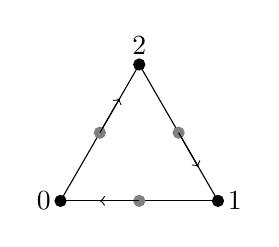
\begin{tikzpicture}
		\draw (0,1.732) -- (1,0);
		\draw (-1,0) -- (1,0);
		\draw (-1,0) -- (0,1.732);
		\filldraw [gray] (-.5,.866) circle (2pt);
		\filldraw [gray] (.5,.866) circle (2pt);
		\filldraw [gray] (0,0) circle (2pt);
		\filldraw [black] (0,1.732) circle (2pt) node[anchor=south]{2};
		\filldraw [black] (1,0) circle (2pt) node[anchor=west]{1};
		\filldraw [black] (-1,0) circle (2pt) node[anchor=east]{0};
		\draw[->] (0,0) -- (-.5,0);
		\draw[->] (-.5,.866) -- (-.25,1.299);
		\draw[->] (.5,.866) -- (.75,.433);
	\end{tikzpicture}
	\caption{The $r$-cyclic assemblage map with duality for $\partial \simplex^2$.}
\end{figure}

\begin{example}\label{example:f3_1}
	For $r=3$, and $a \ot b = [0] \ot [2,1]$ we have:
	\begin{align*}
		f([0] \ot [2,1])
		&= (-1)^{3\cdot 3}g_*\circ s_*^{\Psd}\circ h_*\circ \twist([0] \ot [2,1])
		\\
		&= -g_*\circ s_*^{\Psd}\circ h_*([2,1] \ot [0])
		\\
		&= g_*\circ s_*^{\Psd}\circ h_*([1,2] \ot [0])
		\\
		&= g_*\circ s_*^{\Psd}((0) \ot [0])
		\\
		&= -g_*((0))
		\\
		&= -[0]
	\end{align*}
	Observe that, since the summand $[1,2]$ appears with positive sign in $\partial \sigma = \partial([0,1,2])$, we have that $f([0] \ot \partial\sigma) = [0]$, as dictated by Condition \eqref{cond:1}.
\end{example}

\begin{example}\label{example:f3_2}
	For $r=3$ and $a \ot b = [0,1] \ot [2,0]$, we have:
	\begin{align*}
		f([0,1] \ot [2,0]) &= (-1)^{3\cdot 4}g_*\circ s_*^{\Psd}\circ h_*\circ \twist([0,1] \ot [2,0])
		\\
		&= g_*\circ s_*^{\Psd}\circ h_*([2,0] \ot [0,1])
		\\
		&= -g_*\circ s_*^{\Psd}\circ h_*([0,2] \ot [0,1])
		\\
		&= g_*\circ s_*^{\Psd}((1) \ot [0,1])
		\\
		&= -g_*\circ s_*^{\Psd}((1) \ot [1,0])
		\\
		&= -g_*((1 \subset 01))
		\\
		&= -[1,0]
		\\
		&= [0,1]
	\end{align*}
	Observe that this exhibits Condition \eqref{cond:1} and Condition \eqref{cond:2}:
	\begin{align*}
		f([0,1] \ot \partial\sigma) &= [0,1]
		&
		f(\partial\sigma \ot [2,0]) &= \rho[2,0].
	\end{align*}
\end{example}

\begin{example}\label{example:f5_1}
	For $r=5$ and the first $r$-cyclic straightening of Example \ref{example:asymmetries5}, if $a \ot b = [2,3,0] \ot [4,1,3]$, we have:
	\begin{align*}
		f([2,3,0] \ot [4,1,3]) &= (-1)^{5\cdot 6}g_*\circ s_*^{\Psd}\circ h_*\circ \twist([2,3,0] \ot [4,1,3])
		\\
		&= -g_*\circ s_*^{\Psd}\circ h_*([4,1,3] \ot [2,3,0])
		\\
		&= g_*\circ s_*^{\Psd}((0,2) \ot [2,3,0])
		\\
		&= g_*\circ s_*^{\Psd}((0,2) \ot [0,2,3])
		\\
		&= g_*((02 \subset 023))
		\\
		&= [0,2]
	\end{align*}
\end{example}

\begin{example}\label{example:f5_2}
	For $r=5$ and the first $r$-cyclic straightening of Example \ref{example:asymmetries5}, if $a \ot b = [1,2,3,4] \ot [0,1,2]$ we have:
	\begin{align*}
		f([1,2,3,4] \ot [0,1,2])
		&= (-1)^{5\cdot 7}g_*\circ s_*^{\Psd}\circ h_*\circ \twist([1,2,3,4] \ot [0,1,2])
		\\
		&= -g_*\circ s_*^{\Psd}\circ h_*([0,1,2] \ot [1,2,3,4])
		\\
		&= -g_*\circ s_*^{\Psd}((3,4) \ot [1,2,3,4])
		\\
		&= -g_*\circ s_*^{\Psd}((3,4) \ot [3,4,1,2])
		\\
		&= g_*((34 \subset 134 \subset 1234)) - g_*((34 \subset 234 \subset 1234))
		\\
		&= [3,3,1] - [3,2,1]
		\\
		&= [1,2,3]
	\end{align*}
	Observe that this exhibits Condition \eqref{cond:2}: $f(\partial\sigma \ot [0,1,2] = [1,2,3])$.
\end{example}

